% !TeX spellcheck = en_US

\documentclass[draft=true
,paper=a4
,twoside=false
,fontsize=11pt
,headsepline
,BCOR10mm
,DIV11
]{scrbook}
\usepackage[english, ngerman]{babel}
%% see http://www.tex.ac.uk/cgi-bin/texfaq2html?label=uselmfonts

% define \mysharp using the arev package
\usepackage{arev}
\newsavebox{\sharpbox}
\sbox{\sharpbox}{$\sharp$}
\newcommand{\mysharp}{\usebox{\sharpbox}}

\usepackage[T1]{fontenc}
\usepackage[utf8]{inputenc}
\usepackage{libertine}
\usepackage{pifont}
\usepackage{microtype}
\usepackage{textcomp}
\usepackage[german,refpage]{nomencl}
\usepackage{setspace}
\usepackage{makeidx}
\usepackage{listings}
\usepackage{natbib}
\usepackage[english,colorlinks=true]{hyperref}
\usepackage{soul}
\usepackage{hawstyle}
\usepackage{float}
\usepackage{csquotes}
\usepackage{tabu}
\usepackage{subcaption}
\usepackage{usecases}
\usepackage{enumitem}

%define JavaScript listing
\lstdefinelanguage{JavaScript}{
	keywords={typeof, new, true, false, catch, function, return, null, catch, switch, var, if, in, while, do, else, case, break},
	keywordstyle=\color{blue}\bfseries,
	ndkeywords={class, export, boolean, throw, implements, import, this},
	ndkeywordstyle=\color{darkgray}\bfseries,
	identifierstyle=\color{black},
	sensitive=false,
	comment=[l]{//},
	morecomment=[s]{/*}{*/},
	commentstyle=\color{purple}\ttfamily,
	stringstyle=\color{red}\ttfamily,
	morestring=[b]',
	morestring=[b]"
}

%% define some colors
\colorlet{BackgroundColor}{gray!20}
\colorlet{KeywordColor}{blue}
\colorlet{CommentColor}{black!60}
%% for tables
\colorlet{HeadColor}{gray!60}
\colorlet{Color1}{blue!10}
\colorlet{Color2}{white}

%% configure colors
\HAWifprinter{
	\colorlet{BackgroundColor}{gray!20}
	\colorlet{KeywordColor}{black}
	\colorlet{CommentColor}{gray}
	% for tables
	\colorlet{HeadColor}{gray!60}
	\colorlet{Color1}{gray!40}
	\colorlet{Color2}{white}
}{}
\lstset{%
	numbers=left,
	numberstyle=\tiny,
	stepnumber=1,
	numbersep=5pt,
	basicstyle=\ttfamily\small,
	keywordstyle=\color{KeywordColor}\bfseries,
	identifierstyle=\color{black},
	commentstyle=\color{CommentColor},
	backgroundcolor=\color{BackgroundColor},
	captionpos=b,
	fontadjust=true
}
\lstset{escapeinside={(*@}{@*)}, % used to enter latex code inside listings
	morekeywords={uint32_t, int32_t}
}
\ifpdfoutput{
	\hypersetup{bookmarksopen=false,bookmarksnumbered,linktocpage}
}{}

%% more fancy C++
\DeclareRobustCommand{\cxx}{C\raisebox{0.25ex}{{\scriptsize +\kern-0.25ex +}}}

\clubpenalty=10000
\widowpenalty=10000
\displaywidowpenalty=10000

% unknown hyphenations
\hyphenation{
}

%% recalculate text area
\typearea[current]{last}

\makeindex
\makenomenclature

\begin{document}
	\selectlanguage{english}
	
	
	%%%%%
	%% customize (see readme.pdf for supported values)
	\HAWThesisProperties{Author={Lennart Karsten}
		,Title={Transition of a full-stack application to a microservice frontend}
		,EnglishTitle={Technological evaluation of the MARS Websuite, in a Microservice architecture}
		,ThesisType={Project 1}
		,ExaminationType={Masterprüfung}
		,DegreeProgramme={Bachelor of Science Angewandte Informatik}
		,ThesisExperts={Prof. Dr. Clemen}
		,ReleaseDate={\today}
	}
	
	%% title
	\frontmatter
	
	%% output title page
	\maketitle
	
	\onehalfspacing
	
	%% add abstract pages
	%% note: this is one command on multiple lines
	\HAWAbstractPage
	%% English abstract
	{Websuite, Microservices, Architektur}%
	{This work shows the current state of working with geodata in the MARS working group. Based on that, methods of improvement will be suggested and evaluated.}
	
	\newpage
	\singlespacing
	
	\tableofcontents
	\newpage
	%% enable if these lists should be shown on their own page
	%%\listoftables
	%%\listoffigures
	%\lstlistoflistings
	
	%% main
	\mainmatter
	\onehalfspacing
	%% write to the log/stdout
	\typeout{===== File: chapter 1}


	% !TeX spellcheck = en_US

\chapter{Introduction}
 % Introduction
	% !TeX spellcheck = en_US

\chapter{Groundwork}
This chapter covers the basic technologies and terms used throughout the following chapters.



\section{MARS Websuite}
The MARS Websuite is the web application of the MARS working group. It allows the user to prepare and start simulation runs from within the web browser.\\
The original Websuite has a monolithic structure, meaning it is a traditional, single application with many responsibilities, parts and technologies. The new Websuite contains of over 20 independent micro-services.\\
This work focuses on extracting the front-end of the fullstack application into a single micro-service. While doing so, the inherited components are to be reevaluated, redesigned and if needed, rewritten.


\subsection{Data Types}
\label{sec:data-types}
The Websuite supports several data types, which are used to initial the layers inside the actual simulation.

\subsubsection{Table-based}
This import type supports CSV-files with table data that refers to a specific GPS location. An Example would be the starting positions of agents in a model.

\subsubsection{Time-series}
The time-series import supports CSV-files with data that changes over time. An example is data, containing average temperatures per day over the duration of the desired simulation time.

\subsubsection{Geographic-Information-System (GIS)}
Data with a geographical representation can be imported with the GIS import. It supports the most common file types for GEO-processing, which are:
\begin{itemize}
	\item AciiGrid (*.asc)
	\item GeoTIFF (*.tif)
	\item GeoJSON (*.json)
	\item Shapefile (*.shp, *.shx, *.dbf and additional optional files)
\end{itemize}

\subsubsection{Grid-potential-field}
This data type allows the usage of potential-fields, which contains a grid of percentage values. These grids allow the calculation of distances to non moving objects prior to the simulation and hereby reduce simulation time. The file-ending is \textit{.csv}

\subsubsection{Geo-potential-field}
Geo-potential-field is a specialized grid-potential-field that allows the use of GPS coordinates. The file-ending is \textit{.csv}.

\subsubsection{Obstacle}
Obstacle-layer is a gird that contains obstacles. This can be used to limit agent movement. The file-ending is \textit{.csv}.



\section{Micro-services}
\label{sec:micro-services}
Micro-services describes a software architecture, where the software is split up into small, independent components. These components are loosely coupled and communicate over the network. Each so called service runs in its own process and potentially on a different machine.


\subsection{History}
The concept of handling growing complexity in software is not a new one. The first known thoughts about software structure go back to \citeauthor{conway1968committees}'s law \citeyearpar{conway1968committees}. He claims that organizations tend to structure software systems in a way that matches its hierarchy.\\
A more recent approach towards handling complexity is Service-Oriented Architecture (SOA) by \cite{as2005service}. SOA is described as an architecture, were independent services communicate with each other over the network.\\
The term micro-services was introduced by \cite{martinfowler2014microservices}. Their approach is a more specific version of SOA. This is why micro-services are often referred to as \enquote{SOA done right}.\\
Virtual machines allow the virtualization a whole operating system with its hardware. Containerization software like docker, makes it possible to virtualize on a process level. This significantly reduces overhead and allows independent deployments, as a result the popularity of micro-services has strongly increased over the past 2 years.


\subsection{Single responsibility}
Big, monolithic application grow in size and complexity during their existence. This results into higher costs for maintenance and enhancements. Microservices reduce complexity by splitting the application into smaller logical parts.\\
The definition of how small a service has to be varies, \cite{newman2015building} e.g. claims that micro-services should follow the \enquote{Single responsibility} principle by \cite{martin2003agile}. This states that a given component should have only one reason to change, which results in each component having only one responsibility.


\subsection{Autonomy}
Micro-services are loosely coupled, which means that they can be developed and deployed separately. Each service runs in its own process and communicates with other services over the network layer. It is therefore possible to scale up single services, without having to scale the whole application.



\section{AngularJS}
\label{sec:angularjs}
The WebUI front-end is written with the JavaScript framework AngularJS v1.5. Angular was created by Miško Hevery at Brat Tech LLC in the year 2010 and is under active development by Google Inc. \\
The framework extends HTML5 and JavaScript by various paradigms and patterns, in order to make the development of single-page web applications more appealing. The most relevant features are the \textit{Templating Engine}, \textit{Two Way Data-Binding}, \textit{Model–view–viewmodel} and \textit{Dependency Injection}.


\subsection{Template Engine}
The Angular template is the HTML code, written by the developer. Angular combines this HTML with the model data to render a dynamic view. It has the following features.

\subsubsection{Directives}
Directives are Angular's method of extending HTML by new elements with JavaScript logic attached. This can be used to create reusable, parameterized components.

\subsubsection{Markup}
The templating engine allows the user to reference models from the controller to enrich the HTML with model data. This i done with the double curly brackets notation.

\subsubsection{Filter}
Filters allow formating of input data inside the HTML. Angular has build-in filters for common tasks like formating \textit{numbers} \textit{currencies} or \textit{dates} as well as converters to \textit{uppercase} or \textit{lowercase}. It is also possible to create custom filters based on individual needs.

\subsubsection{Form controls}
The use of form controls allows the validation of form-data in real time. Form elements can be validated against certain gates to detect false user input before it is sent to the back-end.\\
This is possible, because every form field has a JavaScript class that holds validation data. Also CSS error classes exist, which allow to easily visualize false inputs.


\subsection{Model–view–viewModel (MVVM)}
Angular takes advantage of the \textit{Model View Controller} (MVC) pattern, which separates the model that holds the data, the view that is displayed to the user and the controller that holds the logic.\\
Angular's implementation is closer to an Model–view–viewModel (MVVM) approach, because it uses a viewModel inside the controller component. Besides containing the controller logic, the viewModel also holds functions for converting data, which keeps the view clean of logic.

\subsubsection{Model}
The Model  is responsible for storing the current state of the application.

\subsubsection{View}
The View is the HTML, that exists, once Angular has interpreted the template and the appertaining data.

\subsubsection{ViewModel}
\label{sec:viewModel}
The viewModel manages data consistency between the model and view. The Controller sets the initial state of the ViewModel and adds values and functions to it. This added functionality defines the behavior of the application. Inside the view, data can also be read and altered. This data is propagated back to the model.


\subsection{Two Way Data-Binding}
\label{sec:tw-binding}
Angular's two way data-binding is responsible for the communication of MVVM components. The data is bound to a Model, which always holds the most recent state of the application. Changes to the data are always passed to the model and read from it. This means that the controller and the view always operate on the same state. This process is visualized in figure \ref{fig:tw-databinding}.\\
The need to write boilerplate code, for transferring states between the HTML view and the JavaScript controller is hereby removed.

\begin{figure}[H]
	\centering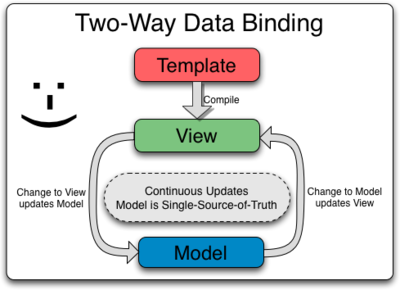
\includegraphics[width=0.5\textwidth]{res/Two_Way_Data_Binding}
	\caption{AngularJS two-way data binding: \url{https://docs.angularjs.org/guide/databinding}}
	\label{fig:tw-databinding}
\end{figure}


\subsection{Dependency Injection (DI)}
Dependency injection (DI) is a specialization of the \textit{inversion of control} pattern and has been named by \cite{fowler2004inversion}. \\
AngularJS adds DI to JavaScript, which allows the integration of dependencies into a specific controller, without making it globally available in the application. This ensures the availability of a component to specific controllers only.\\
It is hereby possible to use existing components and create own modules that can be used anywhere throughout the application. This allows decoupling of components, prevents the necessity for duplicate code and makes it easy to pull in 3rd party dependencies. 


\subsection{Angular Example}
The following example takes advantage of the concepts mentioned in the sections above. \\
Line 2 of listing \ref{lst:angular} defines the \textit{Fruits} factory. It returns a get get function, returning an array of fruits. In line 10, the \textit{FruitCtrl} controller is initiated. It uses dependency injection to take advantage of the Fruits factory. In line 11 the viewModel that is used to communicate with the view, is initiated. The following line adds a \textit{fruits} variable to the viewModel and calls the get function on the injected Fruits.\\
The view in listing \ref{lst:angular-view} specifies the angular app and the controller in line 1. In line 3, the \textit{ng-repeat} directive is used to iterate over the fruits from the viewModel. Listing \ref{lst:angular-result} shows the result.

\begin{lstlisting}[language=javascript, caption=AngularJS directive and controller definition, label=lst:angular]
angular.module("myApp", [])
  .factory('Fruits', function() {
    return {
      get: function() {
        return ["apple", "orange", "raspberry"];
      }
    };
  })
  
  .controller("FruitCtrl", function(Fruits) { // inject Fruits
    var vm = this; // ViewModel
    vm.fruits = Fruits.get(); // call directive
  });
\end{lstlisting}

\begin{lstlisting}[language=html, caption=AngularJS template, label=lst:angular-view]
<div ng-app="myApp" ng-controller="FruitController as fruitCtrl">
  <ul>
    <li ng-repeat="fruit in fruitCtrl.fruits">
      {{fruit}}
    </li>
  </ul>
</div>
\end{lstlisting}

\begin{lstlisting}[language=html, caption=HTML result, label=lst:angular-result]
<ul>
  <li>apple</li>
  <li>orange</li>
  <li>raspberry</li>
</ul>
\end{lstlisting}
 % Groundwork
	% !TeX spellcheck = en_US

\chapter{Analysis}
This chapter is about identifying the requirements, needed to transform the application into a microservice frontend.\\
The Analysis first determines use-cases for the system, based on the stakeholders. These use-cases will be converted into requirements, which are distinguished into functional and non-functional. A gap-analysis is finally performed, to compare requirements of the new system to the old implementation. 


\section{Stakeholders}
Stakeholders are groups of people with an interest in the system. This interest can be from a practical user based standpoint, as well as from a management standpoint.

\subsection{Model Developer}
The Model Developer is a technical user that creates a MARS model in cooperation with a domain expert. His main goal is to make sure the model, he created executes correctly and without errors.

\subsection{Simulation Creator}
The Simulation Creator is a domain expert. He Uses the Model, created by the Model Developer to answer a research question. Model Developers goal is to start various simulations with a given model, to validate or invalidate theories. To do so, he mainly changes the parameters of a given scenario, to find out what their impact on the results are.

\subsection{Group Administrator}
The Group Admin is a user of the system with a leading roll in his group. He wants to manage people belonging to a particular group and handle group dependent settings. He also wants to add users to his group, remove them and handle permissions for data, owned by his group.

\subsection{Administrator}
The Administrator is a global user with far reaching permission inside the system. An admin is able to alter any kind of data inside the system.


\section{Use-cases}
The workflow that includes completing all the necessary steps to start a simulation can be broken down into five parts: \textit{Import Data}, \textit{Check imported Files}, \textit{Create Mapping}, \textit{Start Simulation} and \textit{View Results}. This piece of work does not cover the whole workflow. Instead, it is focused on the first three use-cases.\\
The Use-cases \textit{Manage Groups} and \textit{Manage Users} are for administrative purposes only. They are also not in the scope of this paper.\\
Figure \ref{fig:use-cases} shows an overview of the mentioned use-cases with their stakeholders. Note, that although the Model Developer and the Simulation Creator have a different view of the system, their use-Cases do not differ. This is why they future sections will reference them as users.
\begin{figure}[H]
	\centering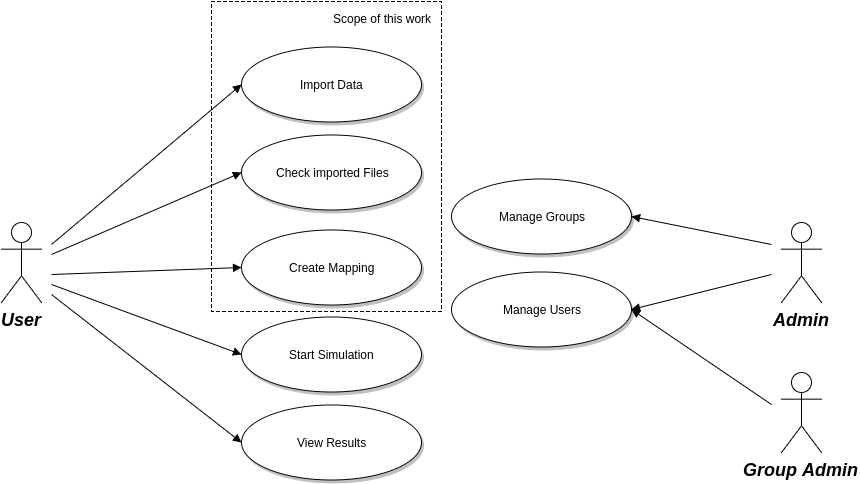
\includegraphics[width=1\textwidth]{res/Use-Cases_reduced}
	\caption{Use-Cases in UML notation}
	\label{fig:use-cases}
\end{figure}

\subsection{Import Files}
\begin{usecase}
	\addtitle{Import I}{Data}
	\addfield{Summary:}{Upload local data files to the Websuite, to use them for a simulation. The following data types have to be supported: 
	\begin{itemize}
		\item Geo-potential-field data
		\item Grid-potential-field data
		\item Obstacle-layer data
		\item Table-based data
		\item Time-series data
		\item GIS data
	\end{itemize}
	}
	\additemizedfield{Actors:}{
		\item User
	}
	\additemizedfield{Preconditions:}{
		\item \textit{Import Data} page is open.
	}
	\additemizedfield{Primary Scenario:}{
		\item The user drags one or multiple files onto the upload window, fills the form for every file and starts the import.
	}
	\additemizedfield{Alternative Scenario:}{
		\item The user clicks the upload button, browses files of his local machine, fills the form for every file and starts the import.
	}
\end{usecase}

\begin{usecase}
	\addtitle{Import II}{Model}
	\addfield{Summary:}{Upload local model files to the Websuite, to use them for a mapping.}
	\additemizedfield{Actors:}{
		\item User
	}
	\additemizedfield{Preconditions:}{
		\item \textit{Import Model} page is open.
	}
	\additemizedfield{Primary Scenario:}{
	\item The user drags one or multiple files onto the upload window, fills the form for every file and starts the import.
	}
	\additemizedfield{Alternative Scenario:}{
		\item The user clicks the upload button, browses files of his local machine, fills the form for every file and starts the import.
	}
\end{usecase}

\begin{usecase}
	\addtitle{Import III}{Bulk}
	\addfield{Summary:}{Upload multible files to the Websuite, with the same metadata, to save time for files that are handled alike.}
	\additemizedfield{Actors:}{
		\item User
	}
	\additemizedfield{Preconditions:}{
		\item \textit{Import Data} page is open.
	}
	\additemizedfield{Primary Scenario:}{
		\item The user drags one or multiple files onto the upload window, fills the one form and starts the import.
	}
	\additemizedfield{Alternative Scenario:}{
		\item The user clicks the upload button, browses files of his local machine, fills the one form and starts the import.
	}
\end{usecase}

\subsection{Check imported Files}
\begin{usecase}
	\addtitle{View I}{Search \& filter results}
	\addfield{Summary:}{Find specific input data with the help of a search and filter functionality.}
	\additemizedfield{Actors:}{
		\item User
	}
	\additemizedfield{Preconditions:}{
		\item \textit{Data View} page is open
		\item Files have been imported
	}
	\additemizedfield{Primary Scenario:}{
		\item The user views imported files, filters them by category and sorts them by name.
	}
	\additemizedfield{Alternative Scenario:}{
		\item The user filters by text input and sorts them by category.
	}
\end{usecase}

\begin{usecase}
	\addtitle{View II}{Check processing result}
	\addfield{Summary:}{Make sure all the imported files from data- and modelimport were processed correctly.}
	\additemizedfield{Actors:}{
		\item User
	}
	\additemizedfield{Preconditions:}{
		\item \textit{Data View} page is open
		\item Files have been imported
	}
	\additemizedfield{Primary Scenario:}{
		\item The user checks the status of multible imported files by searching for them.
	}
	\additemizedfield{Alternative Scenario:}{
		\item none
	}
\end{usecase}

\begin{usecase}
	\addtitle{View III}{View metadata:}
	\addfield{Summary:}{View the metadata of a specific imported file.}
	\additemizedfield{Actors:}{
		\item User
	}
	\additemizedfield{Preconditions:}{
		\item \textit{Data View} page is open
		\item Files have been imported
	}
	\additemizedfield{Primary Scenario:}{
		\item The user clicks on a specific import entry and views the metadata inside a modal window.
	}
	\additemizedfield{Alternative Scenario:}{
		\item none
	}
\end{usecase}

\subsection{Scenario}
\begin{usecase}
	\addtitle{Scenario I}{Create new scenario}
	\addfield{Summary:}{Create a scenario based on a model.}
	\additemizedfield{Actors:}{
		\item User
	}
	\additemizedfield{Preconditions:}{
		\item \textit{Create Scenario} page is open
		\item A model has been uploaded.
	}
	\additemizedfield{Primary Scenario:}{
		\item The user clicks the "add Scenario" button. Inside the new modal, he specifies a name, selects a model and saves the new scenario.
	}
	\additemizedfield{Alternative Scenario:}{
		\item none
	}
\end{usecase}

\begin{usecase}
	\addtitle{Scenario II}{Create scenario as copy}
	\addfield{Summary:}{Create a scenario based on an existing scenario. This clones the original scenario with all its mapping and saves it under a different name.}
	\additemizedfield{Actors:}{
		\item User
	}
	\additemizedfield{Preconditions:}{
		\item \textit{Create Scenario} page is open
		\item A model has been uploaded.
		\item At least one scenario exists.
	}
	\additemizedfield{Primary Scenario:}{
		\item The user clicks the "clone Scenario" button. Inside the new modal, he changes the name and description and saves the new scenario.
	}
	\additemizedfield{Alternative Scenario:}{
		\item none
	}
\end{usecase}

\begin{usecase}
	\addtitle{Scenario III}{Create Mapping}
	\addfield{Summary:}{Combine the fields from the uploaded model with uploaded data.}
	\additemizedfield{Actors}{
		\item User
	}
	\additemizedfield{Preconditions:}{
		\item \textit{Create Mapping} page is open
		\item Data has been imported.
		\item A Model has been imported.
		\item A scenario has been selected.
	}
	\additemizedfield{Primary Scenario:}{
		\item The user connects the required fields to a dataset. He then sets the global parameters for the simulation.
	}
	\additemizedfield{Alternative Scenario:}{
		\item none
	}
\end{usecase}



\section{Requirements}
Derived from the use-cases, the following requirements have been created.


\subsection{Functional Requirements}

\subsubsection{Import}
\reqstartF
\item The webUI has a component that is capable of importing data files for the simulation (data import).
\item The data import supports the \enquote{Geo-potential-field} data type.
\item The data import supports the \enquote{Grid-potential-field} data type.
\item The data import supports the \enquote{Obstacle-layer} data type.
\item The data import supports the \enquote{Table-based} data type.
\item The data import supports the \enquote{Time-series} data type.
\item The data import supports the \enquote{GIS} data type.
\item The data import supports uploading multiple files with the same metadata (bulk upload).
\item The webUI has a component that is capable of importing model files for the simulation (model import).
\item The imports support drag and drop for file selection.
\item The imports support browsing the local computer for file selection.
\item Both imports show the processing of the uploaded files in a view, that is displayed independently of the import page.
\reqendF

\subsubsection{View}
\reqstartF
\item The webUI has a component which allows the user to view the metadata of uploaded files (data view).
\item The data view allows reordering the displayed files.
\item The data view supports filtering the displayed files via text input.
\item The data view supports filtering the displayed files by data type, import status and tag.
\item The data view supports pagination of the displayed data.
\reqendF

\subsubsection{Scenario}
\reqstartF
\item The webUI has a component that allows creating scenarios based on an imported model (Scenario view).
\item The scenario view allows the user to display the already created scenarios.
\item The scenario view allows the user to change the name of a scenario.
\item The scenario view supports duplicating a scenario.
\item Scenarios can be selected from every page.
\reqendF

\subsubsection{Mapping}
\reqstartF
\item The webUI has a component which allows the user to connect uploaded data files to a scenario (mapping view).
\item The mapping view supports transferring multiple mappings of one file to another one.
\item The mapping can be created manually by the user.
\item The mapping view filters the available data files, so only compatible files are shown.
\item The mapping view lets the the user filter compatible mappings by name and tag.
\item When a mapping is created, the next available field is automatically selected.
\item The mapping view renders the correct input type depending on the allowed value (e.g. date-picker for date, checkbox for boolean, etc.).
\item The mapping view shows the validation result from the backend, once a mapping has been saved.
\item The mapping view supports mapping of global parameters.
\item Global scenario parameters can be added and removed by the user.
\reqendF


\subsection{Non-Functional Requirements}
\reqstartNF
\item Input fields for all components only allow the required type of input.
\item The data import and model import share one code base (no duplicate code).
\item Adding new supported data types can be done in one central place.
\item The webUI does not rely on the existence of other services.
\item Errors have to be communicated to the user.
\item The application works in every browser that supports HTML5.
\item No additional software installation is required on the client side.
\item The webUI can be deployed into a Kubernetes cluster.

\reqendNF



\section{Gap-Analysis}
% als Tabelle
 % Analysis
	% !TeX spellcheck = en_US

\chapter{Software Design}
This chapter evaluates the possibility to use microservices for the WebUI components. It also describes the way, the user takes through the system. Finally the REST APIs consumed by the WebUI are described.



\section{Microservices for the WebUI}
\label{sec:MS_for_WebUI}
The MARS Websuite has been transfered into a mircroservice architecture. Backend services communicate via REST instead of local system calls. While this works well for the backend, frontend components behave much different.\\
The code of a backend service is executed in an environment defined by the provider of the application, while the frontend is delivered to the user and executed by his browser. Some browsers don't implement certain features and the implementations might very. As a result, assumptions that made about the software environment, are much weaker. 


\subsection{Constraints}
The constraints mentioned above, brings certain restrictions which are for technical and security reason. They are described in the following section.

\subsubsection{Cross-origin Issue}
Cross-origin requests are API calls to an IP or port other than the one, that provided the original webpage (usually \textit{http\{s\}://localhost/}). These kind of requests can reveal confidential information stored in the session or a cookie inside the browser to a third party.\\
Therefore modern browsers implement the \textit{same-origin policy} as specified in the \textit{RFC 6454 -- The Web Origin Concept} by \cite{barth2011web}, which discourages or blocks cross-origin requests, depending on the browser.\\
Write access to cross-origin locations are excluded, so are certain tags. Among them are \textit{<a>} \textit{<img>}, \textit{<video>}, \textit{<iframe>} and \textit{@font-face}. While not reccomended, it is also possible to deactivate the strict origin policy.

\subsubsection{Only one initial URL}
The user opens a website by typing an URL to the address-bar of his browser. This implies, that one endpoint delivers the whole side. This page has to either load other parts dynamically, or has to aggregate the content of the other frontend microservices in the backend, before it is delivered to the users browser.

\subsubsection{Tightly coupled}
As mentioned in Section \ref{sec:angularjs}, the Websuite consists of an AngularJS single-page application. This implies, that it is indeed a single page, that uses routing to redirect to different pages. That being said, it is not possible to fetch single pages from another service during runtime.

\subsection{Possible Solutions}
The cross-origin issue is quite common for any site that has more than one backend to communicate with. The solution is, to deliver the whole page and all the consumed REST endpoints over a reverse proxy.\\
The harder part is to split up the frontend. To do this, there are a few options.

\subsubsection{AJAX}
This approach delivers an empty page to the user. Afterwards, the client dynamically loads the required sections of a page from different locations, using asynchronous JavaScript calls.\\
This approach requires no backend configuration, since the frontend handles the composition. As a result, many calls to the backend are made, which brings a lot of overhead that impacts performance.

\subsubsection{iFrames}
The iFrame approach renders a frame, that embeds content from a remote location. This is similar to the AJAX approach in the way that it uses client-side composition.\\
The content of the page can not be cached, which reduces performance. Also the content can not control the size of the frame and is not able to communicate with other frames. While workarounds exist, iFrames are a relict from the 90s and are widely unpopular today. It however is still used for a few use-cases, like video embedding from other sites.

\subsubsection{Edge Side Includes}
Edge Side Includes (ESI) is a server-side markup language. It is capable of dynamically adding fragments to one page. As this generates substantial CPU load on the server, a Cache like Varnish is used to make it usable in production. Varnish is one of the few options that supports ESI, which is why, it is the most common choice for ESI.\\
This approach requires a high amount of configuration, to make the Varnish work properly. It includes setting the time-to-live (TTL) for the fragments on the page, based on the content.\\
The way ESI includes resource files like JavaScript, HTML and CSS can not guaranty consistency between the cached versions. This mean that an update in the HTML and JS might deliver the new HTML without the JS, which leads to errors in production.

\subsubsection{Server Side Includes}
Server Side Includes (SSI) is a server-side scripting language supported by the common web-servers like Apache and NGINX, which makes it more accessible than ESI. Caching is mandatory, like it is for ESI, but the lock-in to Varnish does not exist.\\
Unlike ESI, SSI can guarantee the consistency between cached resource files, which makes it a more appealing solution.

%\subsubsection{Compoxure}
%Compoxure is a middleware that tries to serve as an alternative to ESI and SSI with reduced setup afford. It also allows for a more fine-tuned caching of resources. 

\subsubsection{Web Components}
Web Components are a set of features that are being developed as a W3C standard for UI compositions. They consist of the following components.
\begin{itemize}
	\item \textbf{Custom Elements:} Allows creation of custom HTML tags, like Angular's directives.
	\item \textbf{Shadow DOM:} Are elements, located outside the DOM and allow encapsulation of JS or CSS.
	\item \textbf{HTML Import:} Allows including reusable HTML snippets.
	\item \textbf{HTML Template:} Allows to define templates, that are evaluated once they are used. Resources are fetched, once needed.
\end{itemize}

Web Components seem like a promising development towards native support for decoupled frontends. However, the components are still in draft status and are not fully supported by the common browsers jet.


\subsection{general considerations}
Splitting frontends into small services seems like an interesting thought. However, each of the approaches has downsides and that does not even consider some shared issues.\\
Modern frontends require a substantial amount of other code to function. These dependencies are all transfered to the client's browser prior to execution. This requires very strict control of the dependencies and their version to prevent additional load or incompatibilities.\\
For the reasons mentioned above, most cases of composed frontends take advantage of the \textit{Backend for Frontend (BFF)} pattern, which keeps dependencies and code in the frontend to a minimum and builds backends directly tailored to the frontend.\\
The MARS Websuite is not build this way. The backend services provide data and the WebUI contains a lot of logic to prepare and convert data in both directions. The AngularJS framework and its dependencies are not very lightweight either.\\


\subsection{conclusion}
Composing a frontend into multiple parts, requires to consider many aspects. While there are solutions, the afford is not to be underestimated with the currently available technologies. This being said, the effort is only worth it, for very big applications with many developers involved.\\
Moving the MARS WebUI to such a technology would mean to completely rebuild it and reworking the backend services. The afford would be substantial and it is questionable, if the result would be an improvement. The additional complexity introduces potential failures and reduces developers productivity.



\section{Workflow}
To create a successful simulation-run in MARS, certain steps have to be taken. The WebUI implements this workflow from the data import to the execution. Figure \ref{fig:dependency-workflow} shows the single components and the order, they have to executed in.

\begin{figure}[H]
	\centering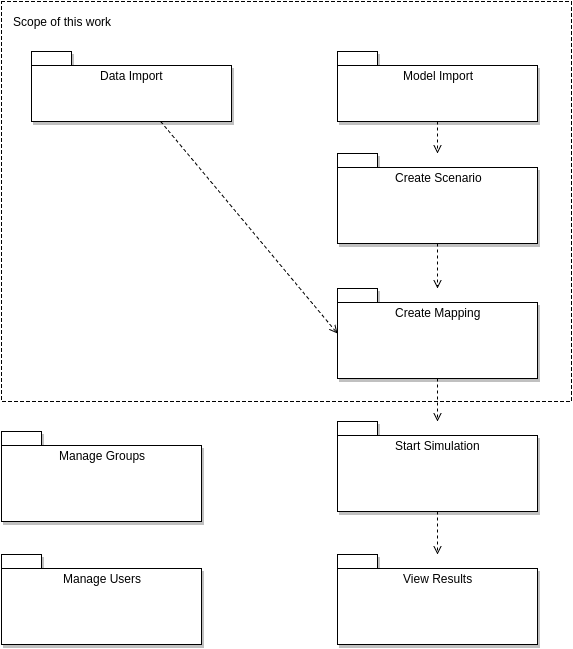
\includegraphics[width=.7\textwidth]{res/Dependency-workflow}
	\caption{Dependency workflow}
	\label{fig:dependency-workflow}
\end{figure}


\subsection{Data Import}
The data import lets the user add files to the system. These files feed the simulation with the information it needs. An example would be a time-series file that contains temperature values over time.\\
The Websuite currently supports the following data types to be added:

\subsubsection{Table-based}
This import type supports CSV-files with table data that refers to a specific GPS location. This could be starting positions of elephants or the position of tree agents in a model.

\subsubsection{Time-series}
The time-series import supports CSV-files with data that changes over time. An example would be a layer containing average temperatures per day.

\subsubsection{Geographic-Information-System (GIS)}
Data with a geographical representation. This can be maps or any of the following data Types:
\begin{itemize}
	\item AciiGrid (*.asc)
	\item GeoTIFF (*.tif)
	\item GeoJSON (*.json)
	\item Shapefile (*.shp and others compressed to a zip-file)
\end{itemize}

\subsubsection{Grid-potential-field}
This data type allows the usage of potential-fields, which contains a grid of percentage values. These grids allow the calculation of distances to non moving objects prior to the simulation and hereby reduce simulation time. The file-ending is \textit{.csv}

\subsubsection{Geo-potential-field}
The Geo-potential-field layer is a specialized grid-potential-field layer that allows the user of GPS coordinates. The file-ending is \textit{.csv}

\subsubsection{Obstacle-layer}
Obstacle-layer is a gird that contains obstacles. This can be used to limit agent movement. The file-ending is \textit{.csv}.


\subsection{Model Import}
The Model Import allows the upload of a zip-file, containing the dlls of the model code. This is used in the scenario creation.


\subsection{Scenario Creation}
This step creates a scenario based on an previously uploaded model. During the creation, the fields that need to be mapped in the following step are determined.


\subsection{Mapping Creation}
Based on the scenario the user maps fields for agents, layers and global parameters to data imported by the data import or to manual values. This data is then validated with the backend. Once the user has mapped all required fields successfully, it is possible to start the simulation.\\
As shown in figure \ref{fig:dependency-workflow} this part will not be covered in this work.



\section{Interface Description}



\subsection{}



\subsection{}



\subsection{}



\subsection{}



\subsection{}



\subsection{}



\subsection{}




% rest Aufrufe % Software Design
	% !TeX spellcheck = en_US

\chapter{Implementation}



\section{Technologies}


\section{Transition of the Components}

\subsection{Import}
\begin{figure}[H]
	\centering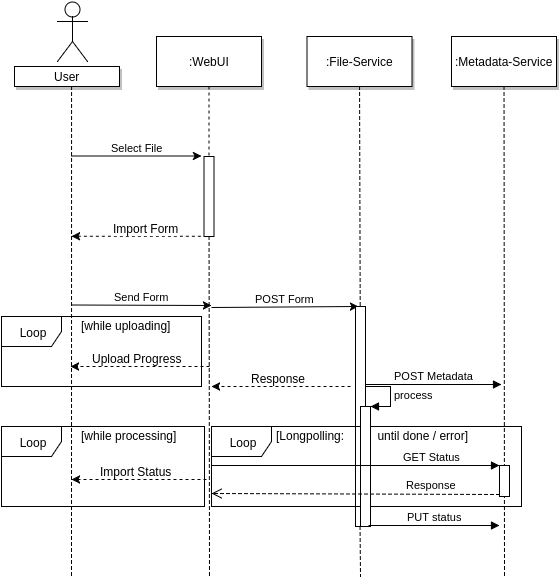
\includegraphics[width=.75\textwidth]{res/Import}
	\caption{Import}
	\label{fig:import}
\end{figure}

\subsection{Data View}

\subsection{Scenario}
\begin{figure}[H]
	\centering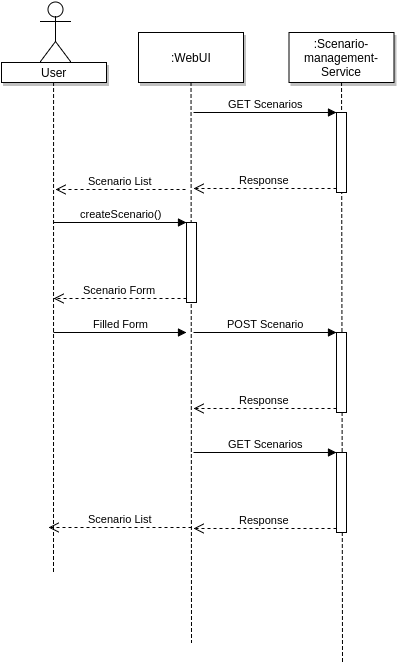
\includegraphics[width=.65\textwidth]{res/Scenario}
	\caption{Scenario}
	\label{fig:scenario}
\end{figure}

\subsection{Mapping}
\begin{figure}[H]
	\centering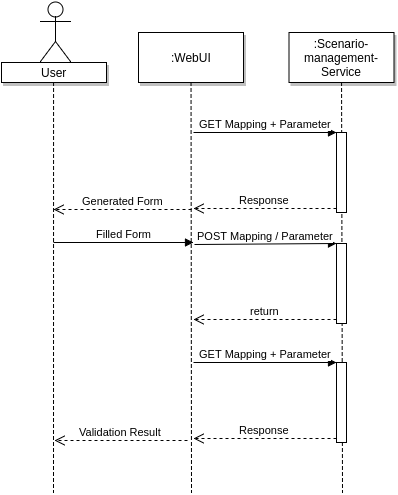
\includegraphics[width=.65\textwidth]{res/Mapping}
	\caption{Mapping}
	\label{fig:mapping}
\end{figure}


\section{Error Handling}
 % Implementation
	% !TeX spellcheck = en_US

\chapter{End}



\section{Summary}
The Monolithic Websuite was transfered into a micro-service based application. This work covered the migration of the front-end into a separate service.\\
The use-cases defined in section \ref{sec:requirements} have been implemented, with few exceptions,  which is still work in progress. The user work-flow is completely implemented and is being used by the model developers. The Tooling of the new WebUI proved to be much more stable, than the old one. Errors during the deployment process are not an issue anymore. Since the migration, the stability of the application has been increased. This is mainly due to the removal of the error prone EdgeJS calls, which have been replaced with properly handled REST calls. The migration of the single components improved the code quality and reduced the amount of technical depth.



\section{Outlook}
The WebUI still lacks a group and user management. A group concept has to be elaborated to allow users to hide their data and results from other users. This can only be guaranteed with an authentication, which uses transport layer encryption and implements best practices for storing confidential user data.
 % End
	
\end{document}